\chapter{Stack}\label{chp:stack}

Stack data structure helps you get the last entered data in O(1) time.
In generally we proces arr[0..idx] elements and push them onto the stack.

\begin{marginfigure}  
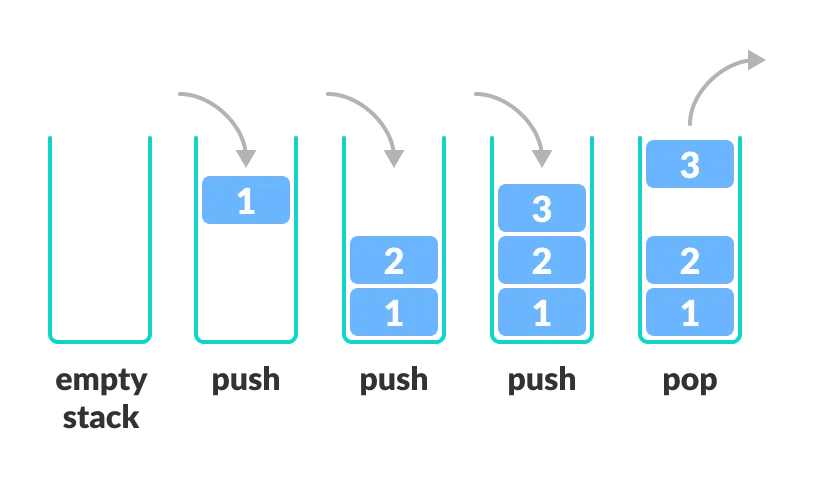
\includegraphics[width=\marginparwidth]{./resources/stack_intro.png}
\caption{stack in action}
\end{marginfigure}

The stack can keep the subsequence or the subarray, depending upon the pop strategy.

Stack is used when you want to have relative sorting of data w.r.t \verb|arr[idx]|

Problems to understand stack.
\begin{exercise}[Fundamental Stack Application Problems.]
    \begin{enumerate}
        \item Rain water harvesting.
        \item Palindromic Check, Longest Palindromic Length
        \item Valid Parenthesis, Longest Valid Parenthesis
        \item Next Greator Element (and related)
        \item all subarray sum(with constrain on max/min element of subarray) without caluclating all subarray. (i.e expected complexiy is linear)
    \end{enumerate}
\end{exercise}

% Pratice problem list
second next Greator
kth next Greator
Widard Strenght.

% TO-DO: Convert marginfigure to a environemtn acceptin g width & hegiht. use xparse package for flexible input

% Include Fils
\import{./}{nge.tex}
% \begin{problem}{Next Greator Element}
    Hello Problem PANKAJ
\end{problem}

Hello, i am PANKAJ Problem sample. % this will work too